\documentclass{article}
\usepackage{amsmath}
\usepackage{enumerate}
\usepackage{listings}
\usepackage{moreverb}
\usepackage[margin=1in]{geometry}
\usepackage{graphicx}
\usepackage{dsfont}
\title{STA 360: Assignment 5}
\author{Michael Lin}

\begin{document}
\maketitle

\begin{enumerate}
\item Let $U$ be a random variable with Uniform(0,1) distribution. Sample a $U$, and suppose for this instance $U=u$. Then set $u$ equal to the c.d.f. of the Gumbel$(c,\beta)$ distribution, i.e.,
\begin{align*}
u &= \exp(-e^{-(x-c)/\beta}) \\
-\log u &= e^{-(x-c)/\beta} \\
\log(\log(1/u)) &= -(x-c)/\beta \\
-\beta\log(\log(1/u)) &=x-c \\
x &= c-\beta \log(\log(1/u))
\end{align*}
Here, $X=x$, and in general, $X$ would be a random variable with Gumbel$(c,\beta)$ distribution.

\item Each of the plot shows that the Monte Carlo approximation for the mean of the Cauchy(0,1) distribution does not converge for large $N$. Even though the mean may appear to converge on an interval, the convergence may be "broken" with a spike despite larger number of samples (it is not clear that the mean will ever converge). This seems to agree with that fact that $\mathds{E}X$ does not exist for the Cauchy distribution. These plots also support the fact that Monte Carlo approximation may not always be suitable for approximation.

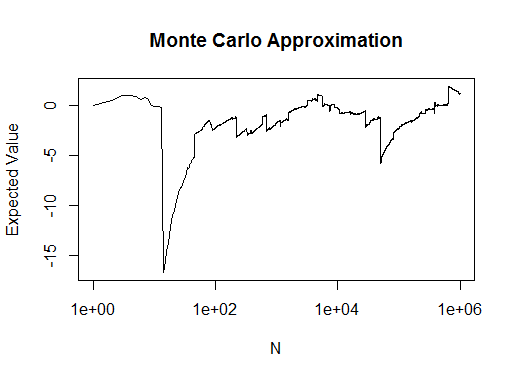
\includegraphics[scale=0.4]{img1.png}
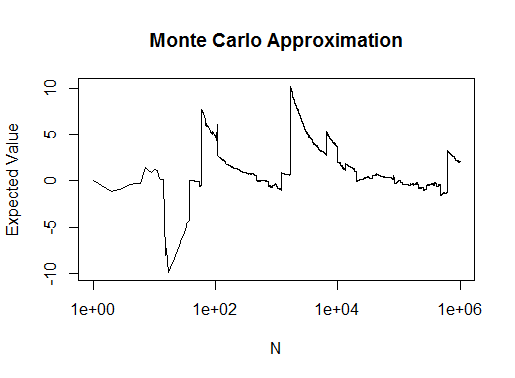
\includegraphics[scale=0.4]{img2.png}\\
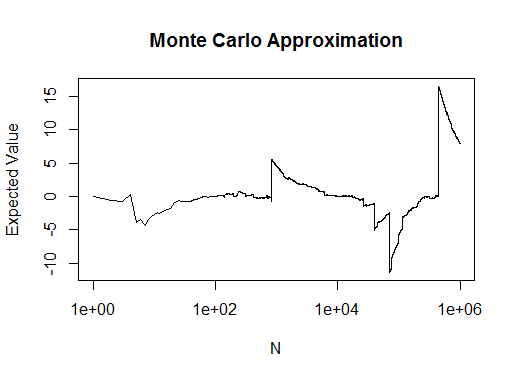
\includegraphics[scale=0.4]{img3.png}
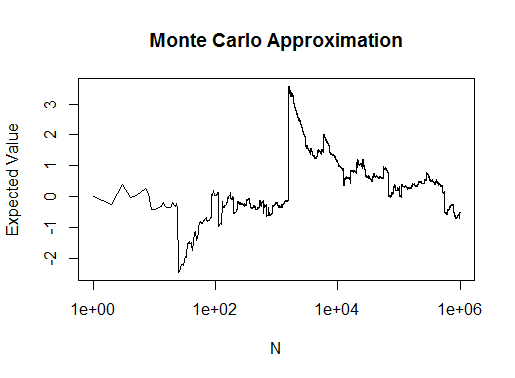
\includegraphics[scale=0.4]{img4.png}

\item Harmonic Mean Approximation
\begin{enumerate}[(a)]
\item We want to show that 
$$p(x_{1:n})\approx \frac{1}{\frac{1}{N}\sum\nolimits_{i=1}^{N}1/p(x_{1:n}|{\bf \theta}_i)} $$
Observe the following:
\begin{align*}
\frac{1}{\frac{1}{N}\sum\nolimits_{i=1}^{N}1/p(x_{1:n}|{\bf \theta}_i)} &\approx \frac{1}{\mathds{E}[\frac{1}{p(x_{1:n}|\theta)}]} \\
&=\Big[\mathds{E}\big[\frac{1}{p(x_{1:n}|\theta)}\big]\Big]^{-1} \\
&=\Big[\int\frac{1}{p(x_{1:n}|\theta)}p(\theta|x_{1:n}) d\theta\Big]^{-1} \\
&=\Big[\int\frac{1}{p(x_{1:n}|\theta)} \frac{p(x_{1:n}|\theta)p(\theta)}{p(x_{1:n})} d\theta  \Big]^{-1} \\
&=\Big[\frac{1}{p(x_{1:n})}\int p(\theta) d\theta  \Big]^{-1} \\
&=\Big[\frac{1}{p(x_{1:n})}\Big]^{-1} \\
&=p(x_{1:n})
\end{align*}
Thus in principle, the harmonic mean approximation converges to the marginal likelihood $p(x_{1:n})$.

\item The harmonic mean approximation for five independent sets returned the following values:
$$\{0.11058598, 0.09973201, 0.10599124, 0.09182709, 0.10342682\}$$
The true value of the marginal likelihood is 0.03891791, and the approximations do not seem to be converging to the true value.

\item The results are similar with a different $\lambda_0$. The true value of the marginal likelihood is 0.003988426 while the harmonic mean approximation returns the following values:
$$\{0.09475517, 0.10211462, 0.02539194, 0.09336356, 0.07787503\}$$
\end{enumerate}

\setcounter{enumi}{4}

\item We want to show that
$$ P(Z \in S) = P(X \in S | X \in A) $$
for all $S\subset A$. For $X\in \mathds{R}^d$, let $a=P(X\notin A)$. Therefore,
\begin{align*}
P(Z\in S) &= P(X_1 \in S) + P(X_1 \notin A, X_2 \in S) + P(X_1 \notin A, X_2\notin A, X_3 \in S)+ \cdots \\
&=P(X_1 \in S) + P(X_1\notin A)P(X_2\in S) + P(X_1 \notin A)P(X_2\notin A)P(X_3\in S) + \cdots \\
&=P(X \in S) + P(X\notin A)P(X\in S) + P(X \notin A)P(X\notin A)P(X\in S) + \cdots \\
&=P(X \in S) + aP(X\in S) + a^2P(X\in S) + \cdots \\
&=P(X \in S) (1+a+a^2+\cdots) \\
&=P(X \in S)\sum\nolimits_{k=0}^{\infty} a^k \\
&=P(X \in S)\frac{1}{1-a} \\
&=P(X \in S)\frac{1}{1-P(X\notin A)} \\
&=P(X \in S)\frac{1}{P(X\in A)} \\
&=P(X \in S | X \in A)
\end{align*}
\end{enumerate}


\pagebreak
R code for number 2:
\listinginput[1]{1}{assign5-2.r}

\pagebreak
R code for number 3:
\listinginput[1]{1}{assign5-3new.r}

\end{document}